\section{Problems}

\noindent {\bf Problem \thesection.\theprob}\stepcounter{prob}

Consider the flow of water in a pipe of $L=100$m, $D=100$mm and the pipe roughness is $e=4$mm. The flow rate is $Q=36.7\,\mathrm{m^3/h}$. Find the pressure drop.

\noindent Solution:
%
\begin{itemize}
\item The flow velocity $v=\frac{36.7}{3600} / \frac{0.1^2\pi}{4}=1.3$m/s.
\item The Reynolds number is $Re=vD/\nu=1.3\times 10^{5}$ (the kinematic viscosity of water is $\nu=10^{-6}\mathrm{m^2/s}$).
\item If the pipe were hydraulically smooth, the friction coefficient would be $\lambda=\frac{0.316}{\sqrt[4]{Re}}=0.0166$.
\item We use the Colebrook-White equation iteratively, starting from $\lambda_0=0.0166$:
	\begin{itemize}
		\item Step 1: $\frac{1}{\sqrt{\lambda_1}}=-2\log_{10}\left(\frac{2.51}{\mathrm{Re}\sqrt{\lambda_0}}+\frac{e}{3.7D}\right)=-2\log_{10}\left(\frac{2.51}{\mathrm{1.3\times 10^{5}}\sqrt{0.0166}}+\frac{4}{3.7\times100}\right)=3.9203$, thus $\lambda_1=0.065$.
		%
		\item Step 2:$\frac{1}{\sqrt{\lambda_1}}=-2\log_{10}\left(\frac{2.51}{\mathrm{Re}\sqrt{\lambda_1}}+\frac{e}{3.7D}\right)=-2\log_{10}\left(\frac{2.51}{\mathrm{1.3\times 10^{5}}\sqrt{0.065}}+\frac{4}{3.7\times100}\right)=3.9262$, thus $\lambda_1=0.0649$. This is reasonably close to $\lambda_1$, hence we stop the iteration.
	\end{itemize}
\item Finally, the pressure drop is $\Delta_p'=\lambda \frac{L}{D}\frac{\rho}{2}v^2=0.0649\frac{100}{0.2}\frac{1000}{2}1.3^2=54.84\mathrm{kPa}=0.548\mathrm{bar}$.
\end{itemize}


\noindent {\bf Problem \thesection.\theprob}\stepcounter{prob}

Calculate the head loss of the pipe depicted in the figure below as a function of the volume flow rate! Parameters: $\zeta_A=1.5$, $\zeta_{B,D}=0.26$, $\zeta_C=0.35$, $\zeta_F=0.36$, $\lambda=0.0155$, $D_s=D_p=D=0.6[m]$ and $Q=0.4[m^3/s]$. 
% 
\begin{figure}[ht]
\begin{center}
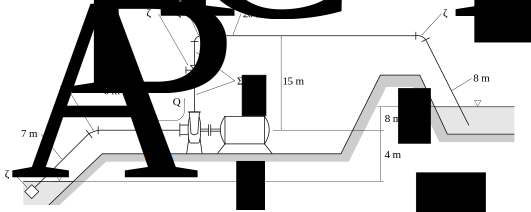
\includegraphics{Problem_solving/figs/PS_HydraulicSystems1.png}
\end{center}
\end{figure}
%
\noindent Solution:
%
\begin{itemize}
\item Static (geodetic) head + dynamic (friction) losses of the pipe: $H_{pipe}=H_{stat}+H_{friction}$
\item Volume flow rate: $Q=c_{s(uction)}A_{pipe,suction}=c_{p(ressure)}A_{pipe,pressure}=c A_{pipe}$
\item The 'extra' $1$ in the pressure side ($...\zeta_D+1$) represents the outflow losses.
\item $H_{stat}=8+4=12[m]$, $L_s=7+6=14[m]$, $L_p=12+20+8=40[m]$
\end{itemize}
%
\begin{alignat*}{1}
H_{pipe}&=H_{stat}+KQ^2= H_{stat}+\left[ \left( \lambda\frac{L_s}{D_s}+\zeta_A+\zeta_B\right)\frac{c_s^2}{2g}\,+\,\left( \lambda\frac{\sum L_p}{D_p}+\zeta_F+\zeta_C+\zeta_D+1\right)\frac{c_p^2}{2g}\right]=\\
%	&=H_{stat}+Q^2\frac{8}{g \pi^2}\left[ \left( \lambda\frac{L_s}{D_s}+\zeta_A+\zeta_B\right)\frac{1}{D_s^4}\,+\,\left( \lambda\frac{\sum L_p}{D_p}+\zeta_F+\zeta_C+\zeta_D+1\right)\frac{1}{D_p^4}\right]=...\\
	&=12[m]+3.25[s^2/m^5] \times Q^2 [m^3/s]^2
\end{alignat*}

%%%%%%%%%%%%%%%%%%%%%%%%%%%%%%%%%%%%%%%%%%%%%%%%%%%%%%%%%%%%%%%%%%%%%%%%%%%%%

\vspace{1cm}
\noindent {\bf Problem \thesection.\theprob}\stepcounter{prob}

The artificial fountain Beneath the St. Gellert  is fed by two pipelines of $30m$ length. The height distance between the pump and the fountain is $22m$. The diameter of the pipes is $D_1=100mm$ and $D_2=70mm$, the friction coefficient of the straight segments is $\lambda=0.02$ and the friction coefficient of the other segments (bends, etc.) is $\zeta=0.5$. Assuming that the flow velocity in the second pipe is $1.5m/s$, calculate the the required head. Calculate the flow velocity in the second pipe and the overall flow rate of the common pump feeding the two pipes.Assuming $65\%$ overall (pump+motor) efficiency, calculate the energy demand for 100 days and the cost of the operation if the energy tariff is $32 HUF/kWh$. (Solution: Without the bypass line: $H=22.826m[$], $Q=0.01678[m^3/s]$, $P=5.78[kW]$ and $Cost=443691HUF$.)

%%%%%%%%%%%%%%%%%%%%%%%%%%%%%%%%%%%%%%%%%%%%%%%%%%%%%%%%%%%%%%%%%%%%%%%%%%%%%%%%%%%
\newpage

\vspace{1cm}
\begin{tcolorbox}
\noindent {\bf Problem \thesection.\theprob}\stepcounter{prob}

A pump delivers $Q=1200[dm^3/min]$ water from an open-surface well, whose water level is $25[m]$ below the default level. The pressure side ends $5[m]$ above the default level and the water flows into an open-surface swimming pool. The diameter of the pipe on the suction side is $D_s=120[mm]$ and $D_p=100[mm]$ on the pressure side. The loss coefficients are $\zeta_s=3.6$ and $\zeta_p=14$ (without the outflow losses). Calculate the required pump head! (Solution: $H_{p,req.}=35.7[m]$) Draw a sketch of the system! (Figure\ref{gen_hs})
\vspace{0.2cm}

Solution:
\vspace{0.2cm}

The points which marked with I and II indicates the beginning and the end of the pump. The whole system is between $1' - 2$ points. The end of the draft tube shall be deep under the fluid surface to avoid the air intake. But in this problem we neglect the x value (the height between the end of the tube and the fluid surface).

Bernoulli equation between $1'$ and $I$: ${e_1}'=e_{I.}+{h_s}'$ it follows ${e_{I.}}'=e_{1}'+{h_s}'$

Bernoulli equation between II and $2$: $e_{II.}=e_2+{h_p}'$, in these formulas, e denotes the “Bernoulli sum” of meter units.The volume flow rate is based on the description of the problem $Q = 1200dm^3/min = 0,02m^3/s$. The head losses for the intake and the delivery ports:
\begin{equation*}
{h_s}'=\zeta_s \frac{{v_s}^2}{2g}=\zeta_s \frac{1}{2g}\frac{Q^2}{{A_s}^2}=3.6\times\frac{1}{2\times 9.81}\times\frac{0.02^2}{\left(0.12^2\times\frac{\pi}{4}\right)}^2=3.6\times\frac{1}{2\times 9.81}\times\frac{0.02^2}{0.01131^2}=0.5738m	
\end{equation*}
\begin{equation*}
{h_p}'=\zeta_p \frac{{v_p}^2}{2g}=\zeta_p \frac{1}{2g}\frac{Q^2}{{A_p}^2}=14\times\frac{1}{2\times 9.81}\times\frac{0.02^2}{\left(0.1^2\times\frac{\pi}{4}\right)}^2=14\times\frac{1}{2\times 9.81}\times\frac{0.02^2}{0.007854^2}=4.627m	
\end{equation*}
\begin{equation*}
v_2=\frac{Q}{A_p}=\frac{0.02}{0.01131}=2.546 m/s	
\end{equation*}
(the specific kinetic energy of the water flow leaving at this speed is lost in the swimming pool (2), its name is the discharge loss,$\frac{v_2^2}{2g}$)
\begin{equation*}
H_{st}=z_2-z_1=25-(-5)=30m \text{  (static head)}	
\end{equation*}
The head of the system (static head+ discharge loss):
\begin{equation*}
H_{system}=H_st+\frac{{v_2}^2}{2g}=30+\frac{2.546^2}{2\times 9.81}=30.33m
\end{equation*}
The head of the pump:
\begin{equation*}
	H_{pump}=e_{II.}-e_{I.}=(e_2+{h_p}')-({e_1}'-{h_s}')=e_2-{e_1}'+{h_p}'+{h_s}'=
\end{equation*}
\begin{equation*}
=\left(\frac{p_2}{\rho g}+\frac{{v_2}^2}{2g}+z_2\right)-\left(\frac{p_{1'}}{\rho g}+\frac{{v_{1'}}^2}{2g}+z_{1'}\right)+{h_p}'+{h_s}'
\end{equation*}
at the surface of the fluid $p_1 = p_0$ (atmospheric pressure), and $v_1 = 0$, because of the relatively large surface of the well, this equation is substituted in the 2nd parentheses of the above equation.
Using that $p_2 = p_0$ is also true:
\begin{equation*}
	H_{sz}=\left(\frac{p_2}{\rho g}+\frac{{v_2}^2}{2g}+z_2\right)-\left(\frac{p_1}{\rho g}+\frac{{v_{1}}^2}{2g}+z_1 \right)+{h_n}'+{h_s}'=\left(\frac{p_0}{\rho g}+\frac{{v_2}^2}{2g}+z_2\right)-\left(\frac{p_{0}}{\rho g}+\frac{0}{2g}+z_1\right)+{h_n}'+{h_s}' 
	\end{equation*}
\begin{equation*}
H_{sz}=\frac{{v_2}^2}{2g}+z_2-z_1+{h_n}'+{h_s}'=35.53m
\end{equation*}
But we can also write that the head of the pump covers the head of the system as well as the losses: $H_{sz}=H_{system}+{h_n}'+{h_s}'=30.33m+4.627m+0.5738m=35.53m$
\end{tcolorbox}

\begin{figure}[ht]
\begin{center}
\includegraphics[scale=0.75]{figs/problem_3p3p34_hyd_sys_fig.png}
\caption{\label{gen_hs}Hydraulic system}
\end{center}
\end{figure}
\vspace{1cm}
\noindent {\bf Problem \thesection.\theprob}\stepcounter{prob}

The submergible pump shown in the picture below delivers $Q = 30 l/s$ water into the basin. The pipe collecting the water of five equal pumps has a diameter $D$. The inner diameter of the pressure tube connecting the pump with the collecting pipe is $d$. Find the Bernoulli enthalpy difference between the two ends of the system, and the pump head! Further data are: $D = 400 mm$, $\lambda_D = 0.018$, $d = 160 mm$, $\lambda_d = 0.021$, $\zeta_{filter} = 3$ , $\zeta_{nrv}=0.25$, $\zeta_{bd} = 0.35$, $\zeta_{2bd} = 0.5$, $\zeta_{bD} = 0.22$. (Solution: $\Delta e_{system}=11.07m$, $H_{pump}=12.80m$)
% 
\begin{figure}[ht]
\begin{center}
\includegraphics{Problem_solving/figs/PS_HydraulicSystems_Submergible.png}
\end{center}
\end{figure}

%%%%%%%%%%%%%%%%%%%%%%%%%%%%%%%%%%%%%%%%%%%%%%%%%%%%%%%%%%%%%%%%%%%%%%%%%%%%%

\vspace{1cm}
\noindent {\bf Problem \thesection.\theprob}\stepcounter{prob}

The head of a 4 stage pump is $68~\mathrm{m}$, the speed of revolution is $1450~\frac{\mathrm{1}}{\mathrm{min}}$. This pump conveys water through a horizontal pipe with diameter $D=120~\mathrm{mm}$. The volumetric flow rate is $0.03~\frac{\mathrm{m^3}}{\mathrm{s}}$. The friction coefficient of the pipe is $\lambda=0.025$. Find the length of the pipe, after which an additional pump needs to be built in the system, if the requirement is that the pressure in the pipe cannot be lower than it is at the suction side! Calculate the same distance in the case when the pipe diameter is $D=160~\mathrm{mm}$! When fewer pumps are in the system, the cost of the investment is obviously lower. Calculate the approximation of the investment cost as a function of the pipe diameter! (hint: the investment cost has two parts: one which is proportional to the pipe length per pump, and another which is proportional to the material cost (thickness of the pipe)). (Solution: $L_1=910.5~\mathrm{m}$, $L_2 = 3835~\mathrm{m}$, $cost=\frac{k_1}{D^5} + k_2 D^2$.)

%%%%%%%%%%%%%%%%%%%%%%%%%%%%%%%%%%%%%%%%%%%%%%%%%%%%%%%%%%%%%%%%%%%%%%%%%%%%%

\vspace{1cm}
\noindent {\bf Problem \thesection.\theprob}\stepcounter{prob}

Find the operation point of a pump which operates a fountain in a lake! The diameter of the pipe at the outlet is $30~\mathrm{mm}$, and the water jet has to reach a height of $20~\mathrm{m}$. The elevation of the jet can be calculated from Newton's law and the gravitational acceleration. However, due to the breaking up of the jet into drops, the jet reaches only $80~\%$ of the theoretical height. At the suction side of the pump, there is a filter, which is characterized by the loss coefficient $\zeta_s=0.7$. At the pressure side, the length of the pipe is $L=1~\mathrm{m}$, the friction coefficient is $\lambda=0.02$, and there are two elbows with loss coefficient $\zeta_e=0.2$ for each of them. The diameter of the pipe at the suction and pressure side is $D=80~\mathrm{mm}$.  Find the specific speed of the pump, if the speed of rotation is $n=1470~\frac{1}{\mathrm{min}}$ and the pump has two stages! Calculate the height of the water jet, if the speed of rotation drops to $n=970~\frac{1}{\mathrm{min}}$! (Solution: $Q=0.01565~\frac{\mathrm{m^3}}{\mathrm{s}}$, $H=25.668~\mathrm{m}$, $n_q=27.13$, $h_{fountain,n=970}=8.71~\mathrm{m}$.)

%%%%%%%%%%%%%%%%%%%%%%%%%%%%%%%%%%%%%%%%%%%%%%%%%%%%%%%%%%%%%%%%%%%%%%%%%%%%%

\vspace{1cm}
\noindent {\bf Problem \thesection.\theprob}\stepcounter{prob}

In a concrete pipe with diameter $D_o = 2800~\mathrm{mm}$ ($\lambda_o=0.03$), there is a smaller pipe with diameter $D_i=1000~\mathrm{mm}$ ($\lambda_i=0.02$). The inner pipe is in the center of the outer pipe. The length of both pipes is $L=540~\mathrm{m}$. The height difference is $\Delta h=3~\mathrm{m}$, and this geodetic head drives the flow. Find the volumetric flow rate
\begin{enumerate}
\item when there is no smaller pipe in the larger pipe and
\item when the smaller pipe is in the larger one!
\end{enumerate}
The friction coefficients should be weighted with the wetted area! (Solution: $Q_1=70713~\frac{\mathrm{m^3}}{\mathrm{h}}$, $Q_2=51830~\frac{\mathrm{m^3}}{\mathrm{h}}$.)
